%!TEX root = CooperBarba-orientation.tex

\subsection{First case: protein G\,B1\,D4$^\prime$} \label{sec:disc_1PGB}

The orientation of protein \gb near charged surfaces was studied using a combined Monte Carlo and molecular dynamics method by Liu and co-workers\cite{LiuLiaoZhou2013} and experimentally by Baio and co-workers.\cite{BaioWeidnerBaughGambleStaytonCastner2012} The availability of these published results was a motivation to use this protein for a first test, to compare with the results obtained with our model. 

The results presented in Figure \ref{fig:1PGB_probability} show that for the most likely orientations, the dipole-moment vector is aligned with the vector normal to the interacting surface. This indicates that the dipole moment is the dominant effect that determines the protein's orientation, over local protein-surface  interactions. This is the expected result, since protein \gb is a relatively small biomolecule. 

Moreover, Figure \ref{fig:1PGB_probability} reveals that protein \gb behaves like a point dipole, as the most likely orientations shift 180$^\circ$ when the sign of the surface charge is flipped. This is also explained by the dipole moment dominating the orientation.
In fact, we repeated this whole set of calculations but placing protein \gb at a greater distance, 5\AA~ away from the surface, and the results did not vary.

The dipolar behavior described by our results agrees with the experiments done by Baio and co-workers, \cite{BaioWeidnerBaughGambleStaytonCastner2012} in which they observed opposite orientations of protein \gb adsorbed on NH$_3^+$ and COO$^-$ self-assembled monolayers. With positively charged surfaces, most of the proteins oriented with the N-terminal of the protein pointing away from the surface, while for negatively charged surfaces the opposite occurred, with the C-terminal pointing away from the surface. This agrees with our results in Figure \ref{fig:1PGB_probability} (the dipole moment vector of protein \gb points from the C-terminal to the N-terminal).

Liu and co-workers \cite{LiuLiaoZhou2013} used a combined Monte Carlo and molecular dynamics method to obtain $<\cos(\alpha_{\text{tilt}})>=0.95$ for $\sigma = 0.05$C/m$^2$, and $<\cos(\alpha_{\text{tilt}})>=-0.85\pm0.05$ for $\sigma = -0.05$C/m$^2$, which agrees well with our results in Table \ref{table:avg}. Note that MD simulations consider van der Waals interactions and conformational changes of the protein, whereas these are not considered in our approach, explaining the slight differences in $<\cos(\alpha_{\text{tilt}})>$.
However, as noted by other researchers,\cite{ZhouChenJiang2003,BaioWeidnerBaughGambleStaytonCastner2012,LiuLiaoZhou2013} electrostatic effects often dominate protein-surface interactions and drive orientation during adsorption, while van der Waals effects play a role only in cases of very low surface charge. For example, in Ref.~\onlinecite{ZhouChenJiang2003}, van der Waals effects were of consequence in a setup with surface charge of 0.006C/m$^{2}$ and high ionic strength, leading to weak electrostatics. In a biosensor-fabrication scenario, this would only be the case with low-quality \sam s.

The results with protein \gb mean that an electrostatic solver with implicit solvent using the Poisson-Boltzmann equation is capable of capturing the driving mechanism of physical adsorption and orientation of the adsorbed molecule, at least in cases where the molecule's dipole moment is dominating the orientation. This is important because protein adsorption, being a free energy-driven process, is difficult to study experimentally\cite{MijajlovicETal2013} and thus simulations offer a promising alternative. Full atomistic molecular dynamics, however, demands large amounts of computing effort, and the possibility of using an electrostatics solver may extend the range of systems that can be investigated.


 \subsection{Second case: immunoglobulin G}

With our numerical model already verified using an analytical solution for spherical geometry\cite{CooperBarba2015a} and the successful results for protein orientation of a small protein near a charged surface (Section \ref{sec:disc_1PGB}), we proceeded to study the effect of surface charge and salt concentration on the orientation of the antibody immunoglobulin G. Antibodies are widely used in biosensors as ligand molecules, due to their affinity and specificity with the target molecule (antigen), and it is vitally important that they are adsorbed on the sensor with the antigen-binding Ig fragment (Fab) pointing away from the sensor, into the oncoming flow containing the antigens (known as ``end-on'' or ``tail-on'' orientation).
Early experimental studies found that antigen/antibody ratio was especially low on negatively charged surfaces,\cite{BuijsETal1997} leading to the notion that protein orientation was affected to leading order by charge. 
One subsequent study\cite{ChenLiuZhouJiang2003} investigated the orientations of two iso-types of immunoglobulin G---\ig 1, corresponding to \pdb\ structure {\small 1IGY}, and \ig 2a, corresponding to \pdb\ {\small 1IGT}---adsorbed on positive and negatively charged surfaces. 
As an indirect method of probing antibody orientation, the researchers obtained adsorbed amounts and antigen/antibody ratios by means of surface-plasmon resonance experiments (e.g., a higher antigen/antibody ratio would indicate that more active sites are accessible and more antibodies are in a favorable orientation). 
The finding was that \ig 1 mainly had a ``head-on'' (unfavorable) orientation on the negatively charged surfaces and a mix of ``tail-on'' (most favorable) and ``side-on'' orientations on the positively charged surfaces. 
\ig 2a, on the other hand, had many orientations on both surfaces with positive and negative charge, leading to the conclusion that \ig 2a is harder to control using electrostatic effects.
Results consistent with these were obtained by Zhou and co-workers\cite{ZhouChenJiang2003} using a united-residue model: a coarse-grained model where each amino-acid is treated as a sphere. They find that \ig 1 will have the favorable ``end-on'' orientation on positive surfaces, as long as the charge density was large enough (0.018C/m$^{2}$, in their case) and the ionic strength was low. But \ig 2a  did not show a clear preferred orientation at the conditions they looked at; the authors attribute this to the weaker dipole moment of this iso-type.
 
We investigated the orientation of \ig 2a, which other studies found harder to orient favorably on a biosensor surface, and used two values of the surface charge ($\sigma=0.05$ and $0.1$C/m$^{2}$) and two values of salt concentration ($\kappa=0.125$ and $0.0625$\AA$^{-1}$), in each case varying two-fold.
 Figures \ref{fig:1IGT_negcharge} and \ref{fig:1IGT_poscharge} present the probability distribution of \ig 2a for many orientations (given by $\alpha_\text{tilt}$ and $\alpha_\text{rot}$), in each case.
 The following discussion refers to each variation of the parameters and the effect on the preferred orientation of the adsorbed antibody and its probability.

 \medskip
 
 \paragraph*{Effect of surface charge---}
 
The lower value of surface charge here is $\sigma=\pm 0.05$C/m$^2$, the same value used in Ref.~\onlinecite{LiuLiaoZhou2013} to mimic the experiments reported in Ref.~\onlinecite{BaioWeidnerBaughGambleStaytonCastner2012}. 
Figures \ref{fig:1IGT_2D_sig-005} and \ref{fig:1IGT_2D_sig005} show that for the lower value of surface charge with the higher salt concentration ($\kappa=0.125$\AA$^{-1}$), there is no clear preferred orientation, to the point that the highest probability falls under 10\%. 
This means that adsorbing the antibodies under these conditions would result in a wide range of orientations, which would not be favorable for biosensor fabrication.
Moreover, the preferred configurations in figures \ref{fig:1IGT_2D_sig-005} and \ref{fig:1IGT_2D_sig005} show the antibody lying flat on the surface, far from the desired ``tail on'' orientation. 
This observation is consistent with a previous study using a unified-residue model,\cite{ZhouChenJiang2003} where this particular antibody showed many possible orientations. 
The authors of that study attributed this behavior to the weaker dipole moment of this molecule, compared with the variant \ig 1.
 
With the higher value of surface charge, in this case $\sigma=\pm0.1$C/m$^2$, the orientation probability distribution in the case of negative charge improves somewhat, as the antibody is slanted sideways rather than lying down for $\kappa=0.125$\AA$^{-1}$ (at least one antingen-binding fragment is pointing up), and the probability of the preferred orientation is almost doubled for low salt concentration, in a ``side on'' orientation.
For positive surface charge the slanted orientation is similar, however the probability is higher for the preferred orientation in both the low- and high-salt cases.
In the cases with higher salt concentration, Figure \ref{fig:1IGT_2D_sig020_kappa01250} shows a preferred orientation with a higher probability of 12\%, compared to 8\% in Figure \ref{fig:1IGT_2D_sig005}, and the dipole moment rotates towards the normal vector. 
For the lower value of salt concentration (Figure \ref{fig:1IGT_2D_sig020_kappa003125}), this effect is smaller, however it shifts the preferred tilt angle in the opposite direction, from $44^{\circ}$ to $64^{\circ}$. Note that the dipole-moment vector does not point straight through the middle between the two Fab fragments, but in an angle.
This indicates that, in contrast to protein \gb, local interactions dominate over the dipole moment. If the dipole moment were the dominant effect, the dipole-moment vector would tend to align to the surface normal as the surface charge increases.
This argues against the suggestion by other researchers\cite{ChenLiuZhouJiang2003,ZhouChenJiang2003} that the dipole-moment vector is the main determinant of orientation.
 
 \medskip
 
 \paragraph*{Effect of salt concentration---}
 
As the surface charge density was varied two-fold, we also varied the Debye length ($\kappa^{-1}$) two-fold. In terms of salt concentration, it means a 4$\times$ decrease in the amount of salt. The higher value of salt concentration corresponds to 145mM, which is in the physiological salt range.  
 
Like increasing the surface charge, lowering the salt concentration affects the orientation probability distribution. 
 For $\sigma=-0.05$C/m$^2$ (Fig.~\ref{fig:1IGT_2D_sig-005_kappa003125}), the effect is a large shift in the preferred tilt angle, from $\alpha_\text{tilt}=116^\circ$ to $\alpha_\text{tilt}=40^\circ$, with a small change in probability. 
For the positive weaker charge, $\sigma=0.05$C/m$^2$ (Fig.~\ref{fig:1IGT_2D_sig005_kappa003125}), not only does the peak probability increase considerably ($\sim 3\times$), but the preferred tilt shifts from $64^{\circ}$ to $44^{\circ}$.
This orientation is favorable for biosensing applications, as the antigen-binding fragments are pointing away from the surface, in a ``tail on'' orientation.
 For the stronger negative charge, $\sigma=-0.1$C/m$^2$, the probability peak increases  $2.5\times$ for a ``side on'' orientation where one of the antigen-binding fragments is attached to the surface in an unfavorable position (Fig.~\ref{fig:1IGT_2D_sig-020_kappa003125}).
 With positive surface charge, the tilt angle shifts in such a way that the antibody is lying on the surface with a marked probability close to $30\%$ (Fig.~\ref{fig:1IGT_2D_sig020_kappa003125}).
 This orientation is not ideal for biosensors, but it is better than the slanted position as neither of the Fabs are attached to the surface.

From the results in Figures \ref{fig:1IGT_negcharge} and \ref{fig:1IGT_poscharge}, we conclude that the iso-type \ig 2a can in general be better orientated with low salt concentration and high surface charge, as we get more pronounced high-probability regions. 
Moreover, good orientations for biosensors are more likely to occur with positive surface charge (Figure \ref{fig:1IGT_3D_sig005_kap003125_til044-rot120}), since the Fab fragments are pointing up.
Previous studies had shown that the \ig 1 variant could be controlled, but not \ig 2a. 
The advantage of a positive surface charge and a low ionic strength had been suggested by previous studies, but not for this particular variant of immunoglobulin G. Note also that our lower value of salt concentration is 37mM, which is a higher amount of salt than other studies.\cite{BuijsETal1997,ChenLiuZhouJiang2003}


 \medskip
A limitation of this study stems from the application of linearized Poisson-Boltzmann equation.
Bu and co-workers\cite{BuVakninTravesset2006} assessed the accuracy of the Poisson-Boltzmann equation for highly charged surfaces ($\sim 0.4$C/m$^2$), getting good agreement with experiments when using a renormalized model. 
Their model uses a renormalized Gouy-Chapman length and boundary condition, but the renormalization factor is close to one in our case. 
Rigorously, the linearized Poisson-Boltzmann equation is a valid approximation of the Poisson-Boltzmann equation when the nondimensional potential is smaller than 1 ($\phi q_e/k_BT<<1$).
However, this restriction can be relaxed when calculating solvation energy. 
For example, we ran a calculation using our boundary element code on an isolated \ig 2a immersed in a solvent with 37mM of salt ($\kappa = 0.0625$\AA$^{-1}$), with the parameters from Table \ref{table:params5}. 
Computing the absolute value of the dimensionless potential on the molecular surface gives over $55\%$ of the triangles with $\phi q_e/k_BT>1$ and an average value of 1.5.
Yet, using the linear or non-linear Poisson-Boltzmann model of APBS,\cite{BakerETal2001} the solvation energy for the isolated \ig 2a gives the same result.
(The APBS tests used a volumetric mesh of $150\times 150\times 150$\AA$^3$ with 449$^3$ nodes.)
Adding a surface with charge $\sigma=0.1$C/m$^2$ next to \ig 2a in the configuration of Fig.~\ref{fig:1IGT_3D_sig02_kap003125_til076-rot160}, the situation is similar: $51\%$ of the triangles have a dimensionless potential with absolute value exceeding 1 and the average is 1.3. By comparison with the isolated \ig 2 case, we expect linearized Poisson Boltzmann to give a good approximation of the solvation energy in this case.
This conclusion is also consistent with the results of Ref.~\onlinecite{Fogolari99} that show good agreement between linear and non-linear Poisson Boltzmann when the average dimensionless potential on the molecular surface is between $-2$ and $2$. 
Finally, with a value of surface charge of 0.1C/m$^2$, the mechanism of protein orientation appears to be dictated by the solvation energy, rather than the surface energy. That is, the maximum probability of the preferred orientation occurs at the minimum of solvation energy.\footnote{See Supplementary Materials.} Since solvation energy in our systems is well approximated by linear PB, we conclude that the use of this theory is justified in these cases.

Our results suggest that a combination of high surface charge and low salt concentration increases the probability of the preferred configuration, and that more favorable orientations are obtained with positive surface charge.
We completed an additional set of tests for the orientation of \ig 2a near a surface with $\sigma =0.2$C/m${^2}$ and $\kappa=0.03125$\AA$^{-1}$, even though the electrostatic potential is outside the linear regime in this case.
The result in Figure \ref{fig:1IGT_sigma02} suggests that as we increase the electrostatic effects, the preferred orientation becomes highly marked, and tends towards a favorable orientation for biosensors.
However, our model is based on the linearized Poisson-Boltzmann equation and this test goes outside the known regime where the model can be applied. We cannot claim that this is a physical situation, but it indicates a trend. Further study of the conditions that make \ig 2a orient favorably for biosensors may need nonlinear models, and combined experimental observations.

\begin{figure*}
   \centering
   \subfloat[Probability distribution]{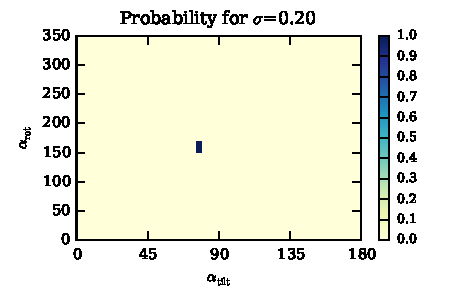
\includegraphics[width=0.4\textwidth]{Figure10a.pdf} \label{fig:1IGT_sig02}}
   \subfloat[x-y plane view for $\alpha_{\text{tilt}} = 76^{\circ}$ and $\alpha_{\text{rot}} = 160^{\circ}$]{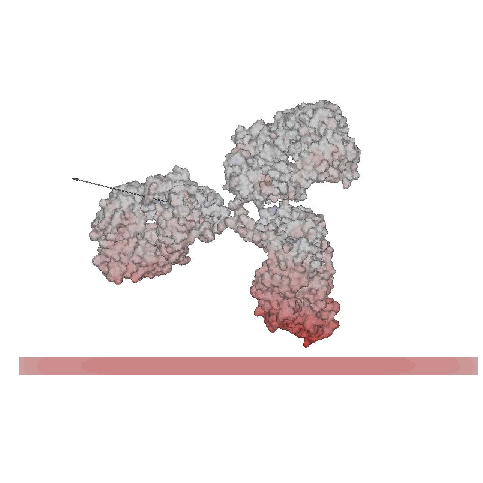
\includegraphics[width=0.4\textwidth]{Figure10b.pdf} \label{fig:1IGT_3D_sig02}}
   \caption{Orientation probability distribution and surface potential of the preferred orientation for immunoglobulin G near a surface with $\sigma=0.2$C/m$^2$ and $\kappa=0.03125$\AA$^{-1}$. Note that these conditions are outside the range of linearized theory (as explained in the Discussion). }
   \label{fig:1IGT_sigma02}
\end{figure*}